% On utilise Beamer (pour faire des slides)
\documentclass[9pt]{beamer}

% Choix du thème
\usetheme{Madrid}

% Packages
\usepackage[utf8]{inputenc}
\usepackage{caption}
\usepackage{pgfpages} 



%%%% Page de garde du document %%%%
\title{Modeleur 3D par B-Mesh}
\author{Julien Daval \\ Omid Ghorreshi}
\institute[Ensimag 2A]{2ème année Ensimag}
\date{11 Juin 2015}
\logo{
\includegraphics[scale=0.3]{images/ensimag.jpg}}


%%%% Début du document %%%%
\begin{document}


%% Affichage de la page de garde
\begin{frame}
	\titlepage
\end{frame}

%% Cadre du projet %%
\begin{frame}
	\frametitle{À propos du projet}
	\framesubtitle{Cadre}
\end{frame}


%% Sommaire
\begin{frame}
	\frametitle{Sommaire}
	\tableofcontents
\end{frame}

%% Pourquoi modéliser avec des sphères ?
\section{Pourquoi modéliser avec des sphères ?}

\begin{frame}
	\frametitle{Sommaire}
	\tableofcontents[currentsection]
\end{frame}

\begin{frame}
	\frametitle{Pourquoi modéliser avec des sphères ?}
	\begin{figure}[H]
		\centering
		\leavevmode
  		\hbox{
  			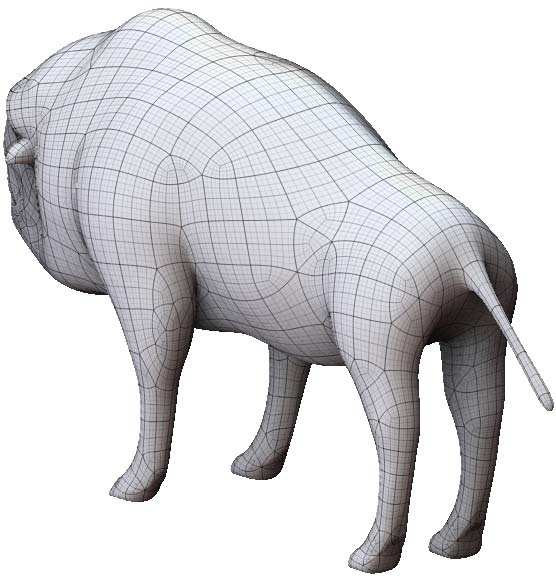
\includegraphics[scale=0.2]{images/basemesh.jpg}
  			\hspace*{0.5cm} 
     		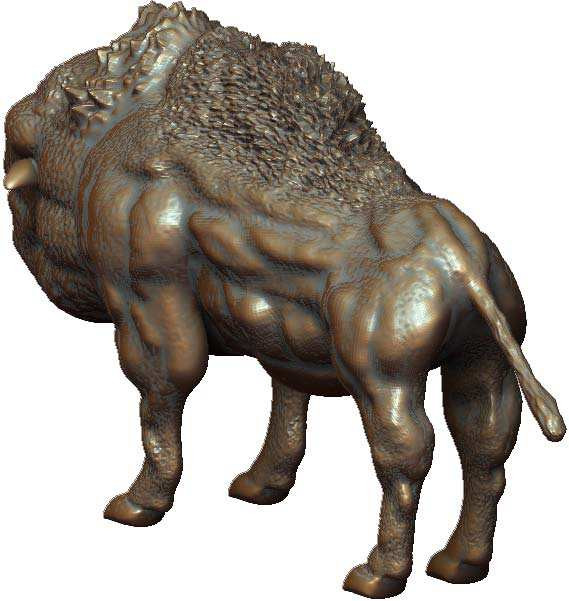
\includegraphics[scale=0.2]{images/detailedmesh.jpg}
     		\hspace*{0.5cm}  
  		}
	\end{figure}
\end{frame}

%% Slide d'introduction
\begin{frame}
	\frametitle{Introduction}
	\begin{block}{Principe du modeleur}
		Générer le maillage d'un objet 3D uniquement à partir de:
		\begin{itemize}
			\item Sphères;
			\item Liens entre ces sphères.
		\end{itemize}
	\end{block}
	
	\begin{center}
		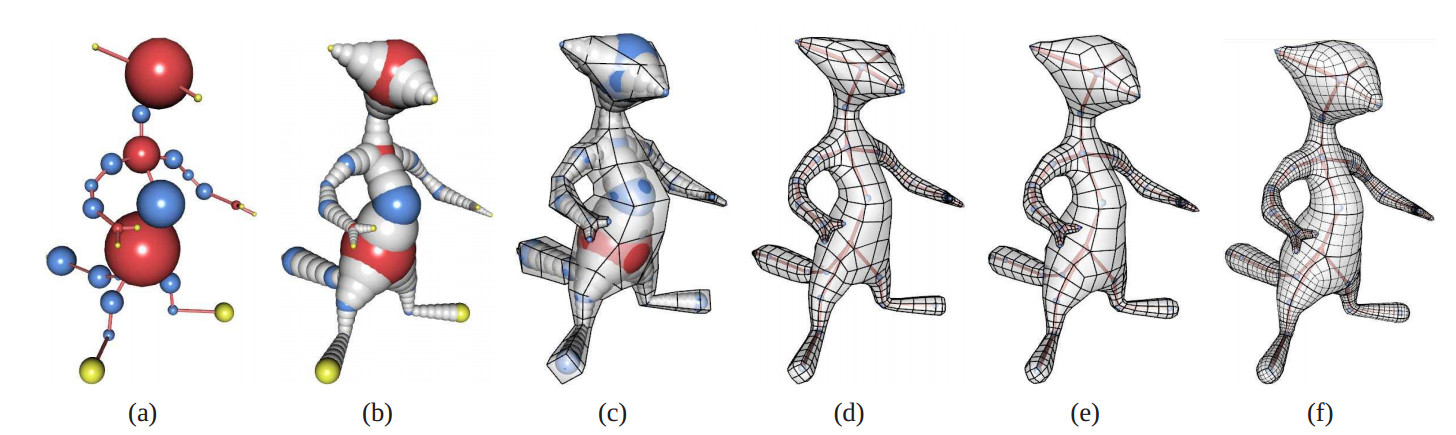
\includegraphics[scale=0.2]{images/bmesh.jpg}
	\end{center}
\end{frame}


%% Interface graphique
\section{Présentation de l'outil}

\begin{frame}
	\frametitle{Sommaire}
	\tableofcontents[currentsection]
\end{frame}

% Slide 1 (screenshot)
\begin{frame}
	\frametitle{Présentation de l'outil}
	\framesubtitle{Aperçu de l'interface graphique}
	\begin{center}
		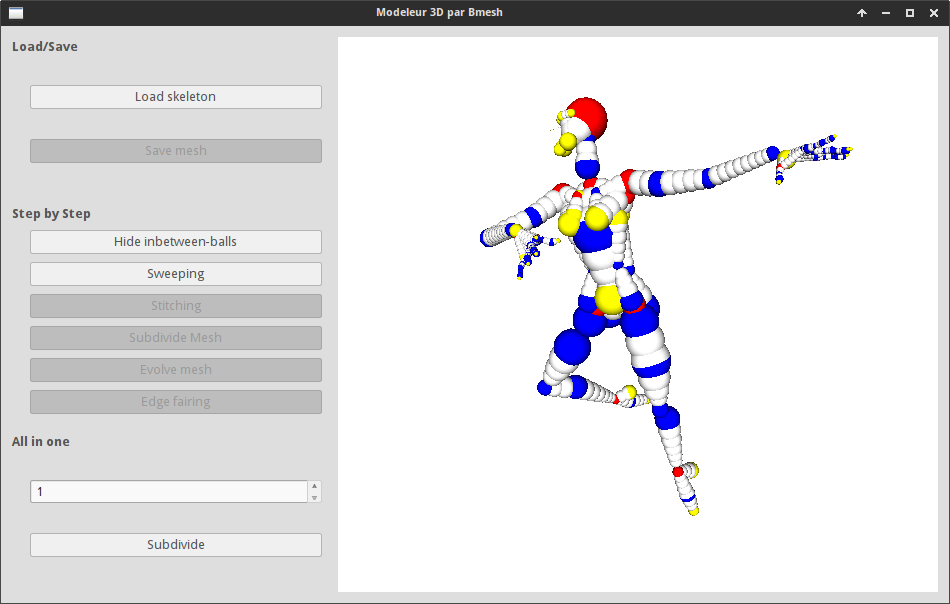
\includegraphics[scale=0.27]{images/screenshot.png}
	\end{center}
\end{frame}

% Slide 2 (description)
\begin{frame}
	\frametitle{Présentation de l'outil}
	\framesubtitle{Fonctionnalités}
	\begin{block}{Chargement / Sauvegarde}
		\begin{itemize}
			\item Chargement d'un squelette (au format .txt)
			\item Sauvegarde du maillage généré (au format .obj)
		\end{itemize}				
	\end{block}
	\begin{block}{Application de l'algorithme}
		\begin{itemize}
			\item Étape par étape...
			\item ... ou tout d'un coup (nombre d'itérations réglable)
		\end{itemize}
	\end{block}
\end{frame}



%% Algorithme
\section{Présentation de l'algorithme}

\begin{frame}
	\frametitle{Sommaire}
	\tableofcontents[currentsection]
\end{frame}

% Intro article
\begin{frame}
	\frametitle{À propos de l'article}
	\begin{block}{Source}
		\begin{center}
			\textit{B-Mesh: A Fast Modeling System for Base Meshes of 3D Articulated Shapes} \\
			Ji Zhongping, Liu Ligang, Wang Yigang \\ 
			
			Institute of Graphics and Image, Hangzhou Dianzi University, China \\
			Department of Mathematics, Zhejiang University, China
		\end{center}
	\end{block}
\end{frame}


%% Tenseur de courbure %%
\begin{frame}
	\frametitle{Tenseur de courbure}
	
	\begin{block}{Définition}
		Courbures et directions principales: valeurs et vecteurs propres de l'endomorphisme symétrique de
		\textbf{Weingarten}
	\end{block}
	
	\begin{block}{Détermination de W}
		\begin{equation*}
			W{(e_i^p)_u \choose (e_i^p)_v} = {(n_i - n_x)_u \choose (n_i - n_x)_v}
		\end{equation*}
		$e_i^p$: projection d'une arête incidente à \textbf{p} dans le plan tangent \\
		$n_i$: normale au point $p_i$ \\
		$((x)_u, (x)_v)$: coordonnées d'un point dans un repère orthonormé du plan tangent
	\end{block}
\end{frame}


%% Subdivision du maillage
\subsection{Subdivision du maillage}
\begin{frame}
	\frametitle{Subdivision du maillage}
	
	\begin{block}{Motivation}
		Avoir un maillage plus fin et plus détaillé
	\end{block}
	
	\begin{block}{Algorithme}
		Algorithme de Catmull-Clark
		\begin{itemize}
			\item algorithme classique;
			\item produit un maillage formé de quadrangles.
		\end{itemize}
	\end{block}
\end{frame}

%% Résultat
\begin{frame}
	\frametitle{Subdivision du maillage}
	\framesubtitle{Résultat}
\end{frame}


%% Mesh evolution %%
\subsection{Évolution du maillage}

%% Résultat: influence de T
\begin{frame}
	\frametitle{Résultats}
	\framesubtitle{Influence de T}
	
	\begin{figure}[H]
		\centering
		\leavevmode
  		\hbox{
  			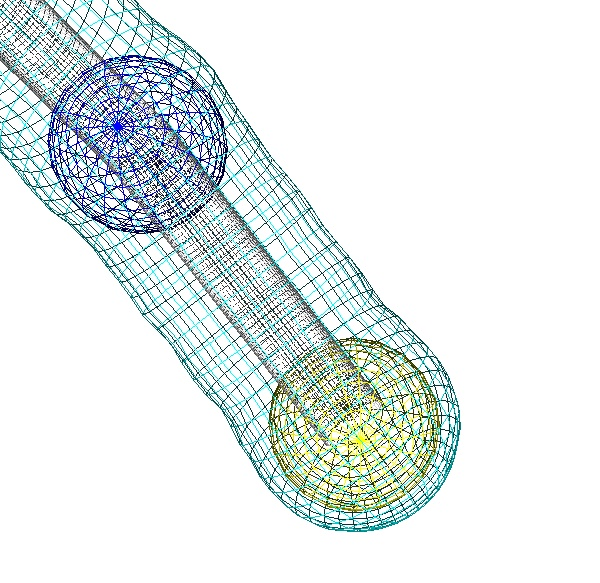
\includegraphics[scale=0.3]{images/evolution_t01.jpg}
  			\hspace*{0.5cm} 
     		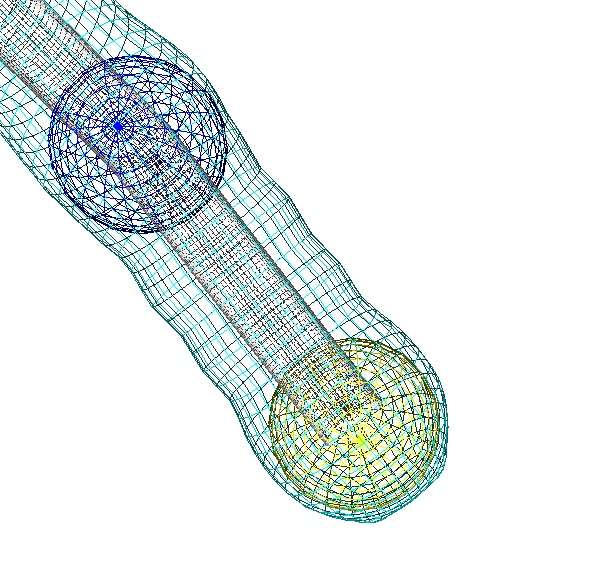
\includegraphics[scale=0.3]{images/evolution_t03.jpg}
     		\hspace*{0.5cm}  
  		}
  		\caption{T = 0.1 (à gauche) et T = 0.3 (à droite)}
	\end{figure}
\end{frame}


%% Edge fairing %%
\subsection{Edge Fairing}

%% Motivation
\begin{frame}
	\frametitle{Edge Fairing}
	\framesubtitle{Motivation}
	
	\begin{block}{Problème de l'évolution}
		Détériore \textit{l'edge flow}
	\end{block}
	
	\begin{block}{Solution ?}
		Appliquer un \textit{fairing} local sur chaque point du maillage.
	\end{block}
	
	\begin{block}{Prérequis}
		Deux types de points:
		\begin{itemize}
			\item les points ayant exactement 4 voisins;
			\item les points n'ayant pas 4 voisins et ceux dont les courbures principales sont identiques.
		\end{itemize}
	\end{block}
\end{frame}

%% Principe
\begin{frame}
	\frametitle{Edge Fairing}
	\framesubtitle{Principe}
	
	\begin{block}{Points de valence 4}
		Pour un point \textbf{p}, minimiser:
		\begin{equation*}
			f(x) = |(a-x).e_v|^2 + |(b-x).e_u|^2 + |(c-x).e_v|^2 + |(d-x).e_u|^2
		\end{equation*}
		avec a,b,c,d projections des voisins de \textbf{p} dans son plan tangent et $e_u, e_v$ directions principales au point 				\textbf{p}
	\end{block}
	
	\begin{block}{Autres points}
		Umbrella operator: approximer le laplacien par $\mathcal{U}(p) = \displaystyle \frac{1}{n} \sum \limits_{i=1}^{n} p_i - p$, avec $p_i$ voisins directs de \textbf{p}.
	\end{block}
\end{frame}

%% Résultats
\begin{frame}
	\frametitle{Edge Fairing}
	\framesubtitle{Résultats}
	
	%% A FAIRE !
\end{frame}






%%%% Fin du document %%%%
\end{document}